% Chapter 1

\chapter{Einführung}
In diesem Kapitel werden wir die zu untersuchende Klein-Gordon-Gleichung (KGG) vorstellen und uns mit den zugehörigen häufig verwendeten Parametern vertraut machen. Anschließend gewinnen wir einen numerischen Lösungsansatz aus der Idee des Operatorsplittings. Die in dieser Arbeit untersuchte \emph{uncertainty} in Gestalt von Zufallsvariablen wird allerdings erst in den folgenden Kapiteln in die KGG einfließen. Zuletzt beschreibt dieses Kapitel relevante Ergebnisse aus der polynomialen Approximationstheorie und bietet einen ersten Einblick in die Beziehung von orthogonalen Polynomen und stochastischen Verteilungen.
\label{Chapter1}

\section{Die Klein-Gordon-Gleichung}
Die für diese Arbeit grundlegende Gleichung ist die lineare Klein-Gordon-Gleichung in der Form
\begin{align}
\label{kgg}
\dtt{u}(t,x)&=\alpha \Laplace_x u(t,x) - \beta(x)u(t,x), \: t>0, \, x\in \Torus^d\\
u(0,x)&=u_0(x), \: x\in \Torus^d\\
\dt{u}(0,x)&=v_0(x), \: x\in \Torus^d
\end{align}
Im Folgenden werden wir auf den, hier zur Betonung verwendeten, Index $x$ des Laplace Operators $\Laplace=\Laplace_x=\frac{\text{d}^2}{\text{d}x^2_1}+\dots+\frac{\text{d}^2}{\text{d}x^2_d}$ verzichten.\\
Bevor wir Abhängigkeiten von einer Zufallsvariablen hinzufügen, ist es hilfreich, die Gleichung für deterministische Parameter besser zu verstehen. Diese Mühe ist nicht vergebens, da einige numerische Verfahren zur Bestimmung der Lösung der zufallsabhängigen Gleichung stark auf einem robusten und schnellen Löser der deterministischen Gleichung basieren. Dazu seien als Stichworte Monte-Carlo-Verfahren und Collocations-Verfahren genannt, die wir im späteren Verlauf genauer betrachten werden.
\subsection{(Physikalische) Definitionen}
Die KGG ist eine relativistische Feldgleichung, welche die Kinematik von spin-freien Teilchen, wie dem Pion, beschreibt. Auch das 2012 entdeckte Higgs-Boson ist ein spin-freies Teilchen, es ist jedoch noch unklar, ob es wirklich das von dem Standardmodell der Teilchenphysik vorgesagte ist und sich vom Standardmodell beschreiben lässt \autocite{cern2016}.\\
Dabei ist
\begin{itemize}
\item $\Torus=\R/(2\pi\Z)$ der skalierte eindimensionale Torus. Wir werden ab sofort die vereinfachte Darstellung $\Torus^d=(-\pi,\pi)^d$ mit periodischen Randbedingungen verwenden. Diese Skalierung des Torus ermöglicht das direkte Verwenden der schnellen Fouriertransformation ohne weitere Skalierung, ist jedoch keine Beschränkung der Allgemeinheit. 
\item die periodische Randbedingung eine vereinfachte Beschreibung des Verhaltens der Lösung ohne Einflüsse von Rändern. Solche Einflüsse, wie sie beispielsweise bei Dirichlet- oder Neumann-Randwerten auftreten, werden vernachlässigt und die Lösung als auf einem großen Träger lebend betrachtet.
\item $\absolute{u(t,x)}^2$ physikalisch als Ladungsdichte des Teilchens zum Zeitpunkt $t$ und Ort $x$ interpretierbar \autocite{kleingordon2016}. 
\item $\alpha>0$ das Quadrat der Wellengeschwindigkeit.
\item $\beta(x)>0, \forall x\in \Torus^d,$ in der physikalischen Interpretation das Quadrat aus einer Kombination von Wellengeschwindigkeit, Masse und planckschem Wirkungsquantum. Die Abhängigkeit des Potentialteils der KGG vom Ort $x$ ist dabei eine Verallgemeinerung der klassischen Gleichung.
\end{itemize}
Wir betrachten im Gegensatz zur physikalischen Darstellung nur reellwertige Funktionen $u$, $u_0$ und $v_0$ und fordern (implizit), dass die Anfangswerte $u_0$ und $v_0$ periodisch in $(-\pi,\pi)$ sind. \todo{(Reelle) Existenztheorie?}

\subsection{Exakte Lösungen}
Für spezielle Konfigurationen der Parameter und Anfangswerte können wir exakte Lösungen angeben. Diese sind hilfreich, um die Korrektheit von Implementierungen schnell und zuverlässig testen zu können. Außerdem zeigen sich so schnell die Grenzen und eventuelle Schwächen der Verfahren für gut gestellte Probleme auf.\\[1cm]
Mithilfe des Separationsansatzes $u(t,x)=g(x)f(t)$ ergibt sich aus (\ref{kgg}) 
\begin{equation*}
(\alpha\Laplace g(x)-\beta(x)g(x))f(t) = g(x)f''(t)
\end{equation*}
womit sich aus Lösungen von
\begin{align*}
\alpha\Laplace g(x)-\beta(x)g(x)&=\lambda g(x), \: \lambda\in\R\\
\mu f(t)&=f''(t), \: \mu\in \R
\end{align*}
Lösungen der KGG ergeben. Für $\beta(x) \equiv \beta>\absolute{\lambda}$ ergibt sich das Eigenwertproblem $\Laplace g(x)=\frac{\beta + \lambda}{\alpha}g(x)$ mit periodischen Randbedingungen und eine lineare gewöhnliche Differentialgleichung.\\Die Anfangswerte $u_0$ und $v_0$ der KGG werden dann entsprechend passend gewählt.\\[1cm]
Beispiele für exakte Lösungen ($d=1$) sind
\begin{align*}
u(t,x)&=\sin(\lambda x)(c_1 \sin(\mu t) + c_2 \cos(\mu t)), \quad \mu^2=\beta+\alpha \lambda^2\\ 
u(t,x)&=(c_1 \sin(\lambda x) + c_2 \cos(\lambda x))\sin(\mu t), \quad \mu^2=\beta+\alpha \lambda^2\\
u(t,x)&=\exp(-\cos(x))\sin(\mu t), \quad \beta(x)=\mu^2+\cos(x)+\sin^2(x), \, \mu \in \R
\end{align*}
wobei $\lambda\in \pi\Z$ um die Periodizität zu gewährleisten und $c_1, c_2 \in \R$ frei wählbare Skalierungsfaktoren.\\
Diese lassen sich auch auf höhere Dimensionen erweitern, beispielsweise
\begin{eqnarray}
u(t,x)=\exp(-\cos(x_1+\dots+x_d))\sin(\mu t)\\
\beta(x)=\mu^2+d(\cos(x_1+\dots+x_d)+\sin^2(x_1+\dots+x_d)), \, \mu\in\R \nonumber
\end{eqnarray}

% Visualize exact solutions by giving two example plots
\begin{figure}[!htb]
\minipage{0.5\textwidth}
  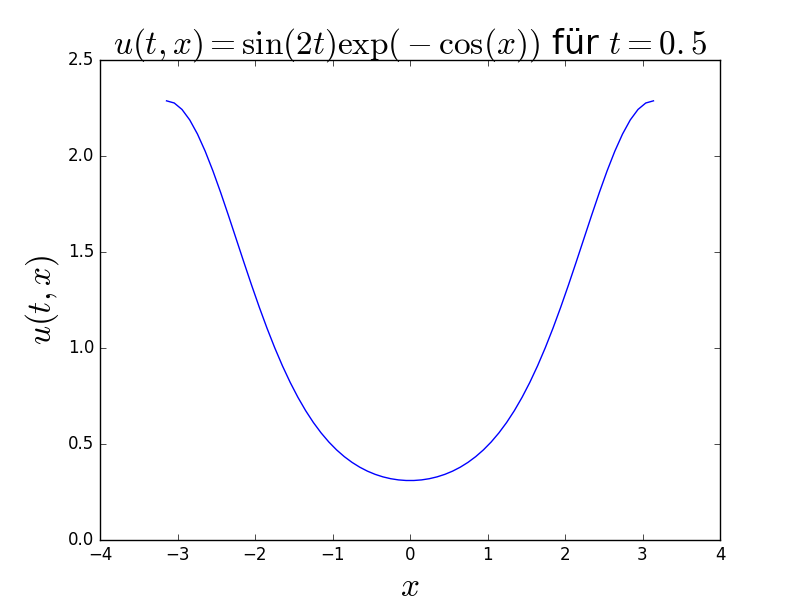
\includegraphics[width=\linewidth]{Figures/kgg_exact_solution_example1d.png}
  \caption{Exakte Lösung für $d=1$}
\endminipage
\minipage{0.5\textwidth}
  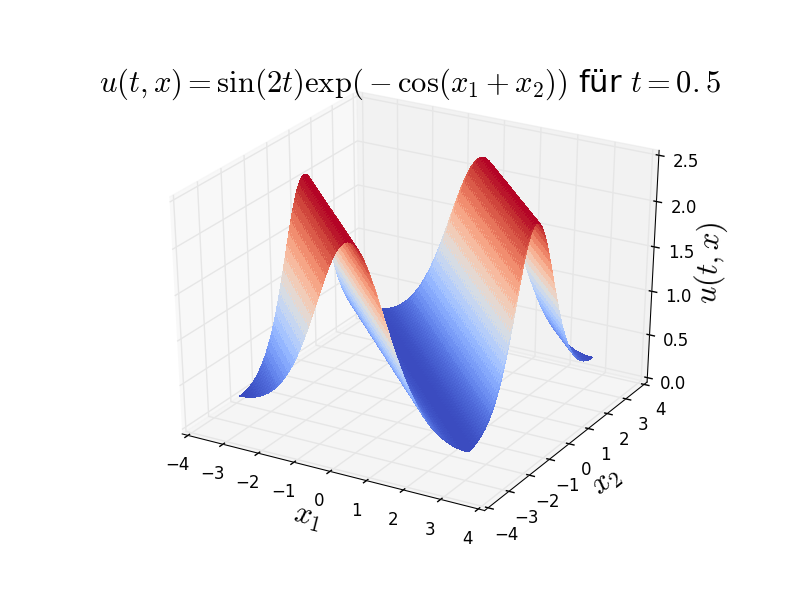
\includegraphics[width=\linewidth]{Figures/kgg_exact_solution_example2d.png}
  \caption{Exakte Lösung für $d=2$}
\endminipage
\captionsetup{labelformat=empty}
\caption{Lösung zum Zeitpunkt $t=0.5$ für die KGG (\ref{kgg}) mit Parametern $\alpha=1$, $
\beta(x)=4+d(\cos(\sum_{j=1}^dx_j)+\sin^2(\sum_{j=1}^dx_j))$.}
\end{figure}

Weitere --allerdings nicht-periodische-- Lösungen finden sich in \autocite{andreipolyanin2004}.

\section{Operatorsplitting}
Um einen Ansatz für numerische Approximationen an die Lösung der KGG zu erhalten bietet sich ein klassischer Operatorsplitting-Ansatz an. Dabei wiederholen wir an dieser Stelle zuerst kurz die relevante Approximationstheorie und diskutieren mögliche Varianten.
\subsection{Generelle Idee}
Angenommen wir stehen vor dem Problem die Differentialgleichung 
\begin{equation}
\label{gencompdgl}
\dt{u}(t)=(L+R)u(t), \, t>0, \quad u(0)=u_0
\end{equation}
zu lösen. Dabei ist im einfachsten Fall $u$ eine vektorwertige Funktion und $L$ bzw. $R$ zwei Matrizen.\\
Sind aufgrund der Struktur der Matrizen --beispielsweise könnte $L$ eine untere und $R$ eine obere Dreiecksmatrix sein-- die Gleichungen 
\begin{align*}
\dt{v}(t)&=Lv(t), \quad v(0)=v_0\\
\dt{w}(t)&=Rw(t), \quad w(0)=w_0
\end{align*}
deutlich einfacher zu lösen als die Gleichung (\ref{gencompdgl}), so lässt sich aus den Lösungen $v$ und $w$ dennoch eine Approximation an $u$ gewinnen.\\
Wir \emph{teilen} (engl. split) die Gleichung also in zwei neue Gleichungen auf. Häufig lässt sich dann eine der gewonnen Gleichungen sogar exakt lösen. Dieser Ansatz funktioniert auch für (nicht-lineare) Operatoren anstelle von Matrizen.\\
Diese zentrale Idee werden wir verwenden, um die KGG 
\begin{equation*}
\dtt{u}(t,x)=\alpha\Laplace u(t,x)-\beta(x)u(t,x)
\end{equation*}
zu splitten. Dabei wird der Operator $\alpha\Laplace$ in $L$ einfließen und $-\beta(x)$ in $R$. Man beachte jedoch, dass die zeitliche Ableitung zweiter Ordnung von $u$ eine Umschreibung in ein System erster Ordnung erfordert, bevor ein Splittingansatz sinnvoll ist.

\subsection{Lie-Trotter-Splitting}
\label{seclietrotter}
Wir beginnen mit einer rigerosen Einführung in Splittingverfahren. Als zentrales Ergebnis werden wir dabei das Strang-Splitting erhalten, welches einen Fehler $\mathcal{O}(\deltat^2)$ in Abhängigkeit von der Zeitschrittweite $\deltat$ besitzt.\\
Die folgende Einführung ist angelehnt an \autocite{patrickdiplom}, welche wiederum aus \autocite[Kapitel II.3 bis II.5]{HairerLubichWanner} übernommen wurde.
\begin{mathdef}[Fluss einer Differentialgleichung]
Der Fluss $\varphi_t$ einer reversiblen Differentialgleichung
\begin{equation}
\label{orddgl}
\dt{y}=f(y),\quad y(0)\:\text{ gegeben}
\end{equation}
mit $f\colon \R^d\to\R^d$ ist die injektive Abbildung, die einem gegebenen $y_0$ die exakte Lösung $y(t)$ zum Zeitpunkt $t$ zuordnet, wobei $y(0)=y_0$. Also gilt
\begin{equation*}
\varphi_t(y_0)=y(t)\enspace und\enspace y(0)=y_0
\end{equation*}
\end{mathdef}

Um Splittingverfahren von möglichst höher Ordnung zu bekommen ist es wichtig, die einzelnen Teilverfahren bestmöglich zu kombinieren. Hierbei spielt das adjungierte Verfahren eine wichtige Rolle, da es dabei hilft, symmetrisierte Verfahren mit gerader Ordnung zu gewinnen.
\begin{mathdef}[Adjungiertes Verfahren]
Ist $\Phi_{\deltat}\colon\R^d\to\R^d$ ein Einschrittverfahren so definieren wir das adjungierte Verfahren $\Phi_{\deltat}^*$ als das Inverse des Einschrittverfahrens mit negativer Schrittweite $\deltat$, also \[\Phi_{\deltat}^*\coloneqq\Phi_{-\deltat}^{-1}\]
Das bedeutet, dass $y_1=\Phi_{\deltat}^*(y_0)$ implizit durch $\Phi_{-\deltat}(y_1)=y_0$ definiert wird.\\
Ist $\Phi_{\deltat}^*=\Phi_{\deltat}$ so nennen wir das Verfahren symmetrisch.
\end{mathdef}
Beispielsweise sind das explizite Euler Verfahren $\Phi_{\deltat}^E$ und das implizite Euler Verfahren $\Phi_{\deltat}^{IE}$ zueinander adjungiert: 
\[\Phi_{-\deltat}^E(y_1)=y_0\implies y_1+(-\deltat)f(y_1)=y_0\implies y_1=y_0+\deltat f(y_1)=\Phi_{\deltat}^{IE}(y_0)\] \\
Ohne Beweis sei bemerkt, dass $(\Phi_{\deltat}^*)^*=\Phi_{\deltat}$ und 
\begin{equation}
\label{adjlemma}
(\Phi_{\deltat}\circ \Psi_{\deltat})^*=\Psi_{\deltat}^* \circ \Phi_{\deltat}^*
\end{equation}

\begin{mathdef}[Konsistenzordnung]
Wir sagen, dass eine numerische Methode zum Lösen von (\ref{orddgl}) (konsistent) von Ordnung $p$ ist, wenn der lokale Fehler für hinreichend glattes $y$
\[\Phi_{\deltat}(y(t))=\varphi_{\deltat}(y(t))+\mathcal{O}(\deltat^{p+1})\] erfüllt.
\end{mathdef}
\begin{maththeorem}[Ordnung des adjungierten Verfahrens, vgl. 
{\autocite[Theorem II.3.2]{HairerLubichWanner}}]
\label{adjfloworder}
Sei $\varphi_t$ der exakte Fluss von (\ref{orddgl}) und sei $\Phi_{\deltat}$ ein Einschrittverfahren von Ordnung $p$ welches 
\[\Phi_{\deltat}(y_0)=\varphi_{\deltat}(y_0)+C(y_0)\deltat^{p+1}+\mathcal{O}(\deltat^{p+2})\]
erfüllt. Dann ist das adjungierte Verfahren $\Phi_{\deltat}^*$ ebenfalls von Ordnung $p$ und erfüllt
\[\Phi_{\deltat}^*(y_0)=\varphi_{\deltat}(y_0)+(-1)^{p}C(y_0)\deltat^{p+1}+\mathcal{O}(\deltat^{p+2})\]
Ist insbesondere $\Phi_{\deltat}$ symmetrisch, so ist wegen $C(y_0)=(-1)^pC(y_0)$ die Ordnung $p$ gerade.
\end{maththeorem}
Nun zerlegen wir die ursprüngliche Gleichung (\ref{orddgl}) in zwei Teile
\[\dt{y}=f(y)=A(y)+B(y) \]
Das Aufteilen ist hierbei nicht eindeutig! Eine Möglichkeit im zweidimensionalen wäre zum Beispiel: $A=\text{P}_{(1,0)^T}f,\,B=\text{P}_{(0,1)^T}f$, wobei $\text{P}_v$ die Projektion auf $\text{span}(v)$ darstellt. Häufig --ebenso wie in unserem Fall der KGG-- ist die bereits vorhandene natürliche Aufteilung der Summe die Methode der Wahl.\\
Sind nun $\varphi_{\deltat}^A$ und $\varphi_{\deltat}^B$ die exakten Flüsse der Systeme
\begin{align}
\dt{y}&=A(y)\quad \text{und} \label{splitsimple1}\\ 
\dt{y}&=B(y) \label{splitsimple2}
\end{align}
so gewinnen wir daraus ein Verfahren zur Lösung der ursprünglichen Gleichung.\\
Hierzu starten wir von einem gegebenen Anfangswert $y_0$ und lösen das System (\ref{splitsimple1}) um einen Zwischenwert $y_{\onehalf}$ zu erhalten. Verwenden wir diesen als neuen Startwert für das System (\ref{splitsimple2}), so erhalten wir einen daraus einen Wert $y_1$, welcher eine Approximation an die Lösung $\varphi_{\deltat}(y_0)$ des ursprünglichen Systems ist.\\[1cm]
\noindent\begin{minipage}{0.3\textwidth}
\begin{tikzpicture}
  \matrix (m) [matrix of math nodes,row sep=3em,column sep=4em,minimum width=2em]
  {
     \, & y_1 \\
     y_0 & y_{\onehalf} \\};
  \path[-stealth]
    (m-2-1.east|-m-2-2) edge node [below] {$\varphi_{\deltat}^A$} (m-2-2)
    (m-2-2) edge node [right] {$\varphi_{\deltat}^B$} (m-1-2)
    (m-2-1) edge [dashed] node [above left] {$\Phi_{\deltat}$} (m-1-2);
\end{tikzpicture}
\begin{tikzpicture}
  \matrix (m) [matrix of math nodes,row sep=3em,column sep=4em,minimum width=2em]
  {
     y_{\onehalf} & y_1 \\
     y_0 & \, \\};
  \path[-stealth]
    (m-1-1.east|-m-1-2) edge node [above] {$\varphi_{\deltat}^A$} (m-1-2)
    (m-2-1) edge node [left] {$\varphi_{\deltat}^B$} (m-1-1)
    (m-2-1) edge [dashed] node [below right] {$\Phi_{\deltat}^*$} (m-1-2);
\end{tikzpicture}
\end{minipage}%
\hfill%
\begin{minipage}{0.7\textwidth}
Die Reihenfolge $A\to B$ ist willkürlich und kann auch umgekehrt werden. Tatsächlich sind die resultierenden Verfahren zueinander adjungiert wegen (\ref{adjlemma}) und der Tatsache, dass der exakte Fluss wegen $y_1=\varphi_{-\deltat}^{-1}(y_0)=\varphi_{\deltat}^*(y_0)=\varphi_{\deltat}(y_0)$ als symmetrisches Einschrittverfahren auffassbar ist. Kurz:\\
\begin{align}
\label{liesplittings}
\Phi_{\deltat}=\varphi_{\deltat}^B \circ \varphi_{\deltat}^A\\
\Phi_{\deltat}^*=\varphi_{\deltat}^A \circ \varphi_{\deltat}^B\nonumber
\end{align} 
\end{minipage}

\begin{maththeorem}[Ordnung des Lie-Trotter-Splittings]
\label{lieorder1}
Das Lie-Trotter-Splitting $\Phi_{\deltat}=\varphi_{\deltat}^B \circ \varphi_{\deltat}^A$ und sein adjungiertes $\Phi_{\deltat}^*=\varphi_{\deltat}^A \circ \varphi_{\deltat}^B$ sind von Ordnung $p=1$.
\end{maththeorem}
\begin{proof}
Die Taylorreihe von $\varphi_{\deltat}$ lässt sich wegen 
\[\varphi_{\deltat}(y_0)=y(\deltat)=y(0)+\deltat \underbrace{y^\prime(0)}_{=f(y_0)}
+\frac{\deltat^2}{2}\underbrace{y^{\prime\prime}(0)}_{=f^\prime(y_0)y^\prime(0)=f^\prime(y_0)f(y_0)}+\mathcal{O}(\deltat^3)\] darstellen als 
\[\varphi_{\deltat}(y_0)=y_0+\deltat f(y_0)+\frac{\deltat^2}{2}f^\prime(y_0)f(y_0)+\mathcal{O}(\deltat^3)\]
Diese vergleichen wir nun mit der Taylorreihe des Splittings
\begin{align*}
\left(\varphi_{\deltat}^B \circ \varphi_{\deltat}^A\right)(y_0)&=
\varphi_{\deltat}^B\left(y_0+\deltat f^A(y_0)+\frac{\deltat^2}{2}f^{\prime A}(y_0)f^A(y_0)+\mathcal{O}(\deltat^3)\right)\\
&=\left(y_0+\deltat f^A(y_0)+\frac{\deltat^2}{2}f^{\prime A}(y_0)f^A(y_0)\right)
+\deltat f^B\left(y_0+\deltat f^A(y_0)+\mathcal{O}(\deltat^2)\right)\\
&\quad+\frac{\deltat^2}{2}f^{\prime B}\left(y_0+\mathcal{O}(\deltat)\right)f^B\left(y_0+\mathcal{O}(\deltat)\right)+\mathcal{O}(\deltat^3)\\
&=y_0+\deltat f(y_0)+\frac{\deltat^2}{2}f^\prime(y_0)f(y_0)\\
&\quad+\frac{\deltat^2}{2}\left(f^{\prime B}(y_0)f^A(y_0)-f^{\prime A}(y_0)f^B(y_0)\right)+\mathcal{O}(\deltat^3)
\end{align*}
so bekommen wir für hinreichend glatte Funktionen $f^A$, $f^{\prime A}$, $f^B$ und $f^{\prime B}$ den Fehler \[\varphi_{\deltat}(y_0)-\left(\varphi_{\deltat}^B \circ \varphi_{\deltat}^A\right)(y_0)=\mathcal{O}(\deltat^2)\] und die Ordnung $p=1$. Mit Satz \ref{adjfloworder} ist das adjungierte Verfahren ebenfalls von Ordnung $p=1$.
\end{proof}

\subsection{Strang-Splitting}
\label{secstrang}
Durch geschicktes Kombinieren der Einschrittverfahren $\Phi_{\deltat}$ und $\Phi_{\deltat}^*$ mit verschiedenen Schrittweiten lassen sich Splittingverfahren beliebiger Ordnung konstruieren.
\begin{maththeorem}[vgl. {\autocite[Theorem II.4.1ff]{HairerLubichWanner}}]
Ist $\Phi_{\deltat}$ ein Einschrittverfahren von Ordnung $p$ so ist die Zerlegung
\[\Psi_{\deltat}=\Phi_{a_s\deltat}\circ \Phi_{b_s\deltat}^*\circ\dots\circ\Phi_{b_2\deltat}^*\circ\Phi_{a_1\deltat}\circ\Phi_{b_1\deltat}^*\]
von Ordnung $p+1$, wenn 
\begin{align*}
\sum_{j=1}^sa_j+b_j&=1\\
\sum_{j=1}^sa_j^{p+1}+(-1)^pb_j^{p+1}&=0
\end{align*}
\end{maththeorem}
Ohne das allgemeine Ergebnis zu verwenden wollen wir nun dennoch ein Verfahren $\Phi_{\deltat}^S$ mit Ordnung $p=2$ gewinnen. Dieses sollte möglichst den selben Zeitaufwand wie das Lie-Trotter-Splitting besitzen. Hierzu verwenden wir den Ansatz \[\Phi_{\deltat}^S=\Phi_{\deltathalf}^*\circ\Phi_{\deltathalf}\]
Wir erkennen sofort, dass es sich hierbei um ein symmetrisches Verfahren handelt. Als Komposition von Verfahren mit Ordnung 1 (siehe Satz \ref{lieorder1}) ist es ebenfalls mindestens von Ordnung 1. Als zusätzlich symmetrisches Verfahren gilt mit Satz \ref{adjfloworder}, dass das Verfahren mindestens von Ordnung 2 ist.\\
Dieses sogenannte \emph{Strang-Splitting} lässt sich unter Verwendung der aufgeteilten Flüsse (\ref{liesplittings}) auch darstellen als 

\noindent\begin{minipage}{0.3\textwidth}
\begin{tikzpicture}
  \matrix (m) [matrix of math nodes,row sep=3em,column sep=4em,minimum width=2em]
  {
  	 \, & y_{\frac{3}{4}} & y_1\\
     \, & y_{\frac{2}{4}} & \, \\
     y_0 & y_{\frac{1}{4}} & \,\\};
  \path[-stealth]
    (m-3-1.east|-m-3-2) edge node [below] {$\varphi_{\deltathalf}^A$} (m-3-2)
    (m-3-2) edge node [right] {$\varphi_{\deltathalf}^B$} (m-2-2)
    (m-3-1) edge [dashed] node [above left] {$\Phi_{\deltat}$} (m-2-2)
    
    (m-1-2.east|-m-1-3) edge node [above] {$\varphi_{\deltathalf}^A$} (m-1-3)
    (m-2-2) edge node [left] {$\varphi_{\deltathalf}^B$} (m-1-2)
    (m-2-2) edge [dashed] node [below right] {$\Phi_{\deltat}^*$} (m-1-3);
\end{tikzpicture}
\end{minipage}%
\hfill%
\begin{minipage}{0.7\textwidth}
\begin{align}
\Phi_{\deltat}^S&=\varphi_{\deltathalf}^A\circ\varphi_{\deltathalf}^B\circ\varphi_{\deltathalf}^B\circ\varphi_{\deltathalf}^A\nonumber\\
&=\varphi_{\deltathalf}^A\circ\varphi_{\deltat}^B\circ\varphi_{\deltathalf}^A
\end{align}
\end{minipage}
Für einen Schritt ist also nur der anderthalbfache Aufwand nötig wie beim Lie-Trotter-Splitting, aber man gewinnt bereits eine Ordnung dazu. Unter Umständen kann dies sogar noch verbessert werden:\\
Gegeben sei ein Anfangswert $y_0$ für das System (\ref{orddgl}). Ist man an einer Approximation $y_T$ der Lösung $y(T)$ zu einem Zeitpunkt $T=n\deltat>0$ interessiert, so gilt unter Verwendung des Strang-Splittingverfahrens
\begin{align*}
y_T&=\underbrace{\Phi_{\deltat}^S\circ\dots\circ\Phi_{\deltat}^S}_{n\text{ mal}}(y_0)\\
&=\left(\varphi_{\deltathalf}^A\circ\varphi_{\deltat}^B\circ\varphi_{\deltathalf}^A\right)\circ\left(
\varphi_{\deltathalf}^A\circ\varphi_{\deltat}^B\circ\varphi_{\deltathalf}^A\right)\circ\dots\circ\left(
\varphi_{\deltathalf}^A\circ\varphi_{\deltat}^B\circ\varphi_{\deltathalf}^A\right)\\
&=\varphi_{\deltathalf}^A\circ\varphi_{\deltat}^B\circ\left(\varphi_{\deltat}^A\circ\varphi_{\deltat}^B\right)\circ\left(\varphi_{\deltat}^A\circ\varphi_{\deltat}^B\right)\circ\dots\circ\left(\varphi_{\deltat}^A\circ\varphi_{\deltat}^B\right)\circ\varphi_{\deltathalf}^A\\
&=\varphi_{\deltathalf}^A\circ\varphi_{\deltat}^B\circ
\underbrace{\Phi_{\deltat}^*\circ\dots\circ\Phi_{\deltat}^*}_{n-1\text{ mal}}\circ\,\varphi_{\deltathalf}^A
\end{align*}
Durch das Kombinieren der äußeren Halbschritte bekommt man also nun eine Darstellung des Strang-Splittings, die nur einen zusätzlichen Fluss berechnen muss und trotzdem Ordnung $p=2$ besitzt. Man muss hierbei allerdings auf Zwischenergebnisse verzichten, da diese eine weitere Anwendung von $\varphi_{\deltathalf}^A$ benötigen würden.\\[0.5cm]
Bisher sind wir davon ausgegangen, dass sich die Flüsse $\varphi_{\deltat}^A$ btw. $\varphi_{\deltat}^B$ exakt berechnen lassen. Dies ist in den seltensten Fällen der Fall und man verwendet stattdessen approximative Verfahren $\Phi_{\deltat}^A$ bzw. $\Phi_{\deltat}^B$. 
\begin{maththeorem}
Sind die Verfahren ebenfalls von Ordnung $p$, d.h. falls 
\begin{align*}
\Phi_{\deltat}^A(y(t))=\varphi_{\deltat}^A(y(t))+\mathcal{O}(\deltat^{p+1})\\
\Phi_{\deltat}^B(y(t))=\varphi_{\deltat}^B(y(t))+\mathcal{O}(\deltat^{p+1})
\end{align*}
so gelten Satz \ref{adjfloworder}, Satz \ref{lieorder1} und alle entsprechenden Aussagen aus Kapitel \ref{seclietrotter} und Kapitel \ref{secstrang} für $\Phi_{\deltat}^A$ und $\Phi_{\deltat}^B$ anstelle von $\varphi_{\deltat}^A$ und $\varphi_{\deltat}^B$.\\
Insbesondere ist das Strang-Splitting immer noch von Ordnung 2, wenn alle verwendeten Approximationen von Ordnung 2 sind.
\end{maththeorem}
\begin{proof}[Beweisidee]
Am Beispiel von $\varphi_{\deltat}^A$ und $p=1$:\\
Man verwendet die Darstellung $\varphi_{\deltat}^A(y_0)=y_0+\deltat f^A(y_0)+\mathcal{O}(\deltat^2)$ und ersetzt $\varphi_{\deltat}^A$ durch $\Phi_{\deltat}^A$. Die Vorgehensweise in den Beweisen muss dann höchstens minimal angepasst werden.\\
Man beachte hierbei, dass nun $\Phi_{\deltat}^A$ im Gegensatz zu $\varphi_{\deltat}^A$ nicht mehr symmetrisch ist. Die Argumentation über die Ordnung von symmetrischen Verfahren kann also nicht direkt verwendet werden, um $p=2$ für das Strang-Splittings zu begründen. Außerdem kann dies die Möglichkeit, das Strang-Splitting durch Kombination der Halbschritte zu beschleunigen, zunichte machen.
\end{proof}

\subsection{Numerischer Löser der KGG}
Dieser Abschnitt ist das wichtige Fundament, auf dem viele numerischen Lösungsverfahren basieren werden. Um ein Operator Splitting auf die KGG anwenden zu können, muss diese zuerst in eine Gleichung mit Zeitableitung erster Ordnung in der Form von (\ref{orddgl}) umgeschrieben werden. Formal:
\begin{align}
\dtt{u}(t,x)&=\alpha \Laplace u(t,x) - \beta(x)u(t,x)\nonumber\\
\iff
\dt{\begin{pmatrix}
u\\
v
\end{pmatrix}}(t,x)&=
\begin{pmatrix}
0 & I\\
\alpha \Laplace - \beta(x) & 0
\end{pmatrix}
\begin{pmatrix}u\\v\end{pmatrix}(t,x)\nonumber\\
\label{eqn:formalsplit_kgg}
&=\left[\begin{pmatrix} 0 & wI\\ \alpha \Laplace & 0\end{pmatrix} 
+ \begin{pmatrix} 0 & (1-w)I\\ -\beta(x) & 0\end{pmatrix}\right]
\begin{pmatrix}u\\v\end{pmatrix}(t,x)
\end{align}
für ein Gewicht $w\in [0,1]$. Doch bevor wir dies als Grundlage für ein Splitting verwenden, müssen wir den Operator $\Laplace$ genauer untersuchen.
\subsubsection*{Ortsdiskretisierung durch Fourier Pseudo-Spectral Methode}
Um einen numerischen Zugang zum Laplace Operator $\Laplace$ zu bekommen, benötigen wir zuerst eine Diskretisierung des Ortes $x_j=-\pi+2\pi\frac{j}{N}\in [-\pi,\pi)$ für $j=0,\dots,N-1$ und $N\in\N$. Da wir periodische Lösungen $u$ der KGG suchen, bietet es sich an, die endliche Fourier-Approximation von $u$ zu verwenden. Wir werden den Ansatz zuerst ausführlich für $d=1$ erläutern und später die Verallgemeinerung auf höhere Dimensionen aufzeigen.\\
Die Fourier-Approximation ist für jedes $t>0$, $N\in 2\N$ und eine Indexmenge $\mathcal{I}_N=\left\lbrace -\frac{N}{2},\dots,-1,0,1,\dots,\frac{N}{2}-1\right\rbrace$ definiert durch
\begin{equation}
\label{eqn:fourier_approx}
u(t,x)\approx \sum_{k\in\mathcal{I}_N}\fourier{u}_k(t)e^{ikx}, \quad x\in\Torus^d
\end{equation}
wobei für die Fourier-Koeffizienten $\fourier{u}_k(t)=\frac{1}{2\pi}\int_{-\pi}^\pi u(t,x)e^{-ikx}dx\in\Complex$ gilt. \\
Um die Konvergenz der Fourier-Approximation einer Funktion zu erhalten, benötigen wir gewisse Anforderungen an die Glattheit der Funktion. Dabei ist bereits Stetigkeit und stückweise stetige Differenzierbarkeit ausreichend für eine gleichförmige Konvergenz. 
\begin{mathbsp}
Als Demonstration der Konvergenz der Fourierapproximation und der Möglichkeit, Ableitungen im Fourierraum durchzuführen, seien an dieser Stelle zwei Beispiele gemacht.\\
Wir betrachten zu einer periodischen Funktion $f\colon\Torus\to\R$ die diskrete Fourierapproximation
\[f(x)\approx \sum_{k=-N}^N\fourier{f}_ke^{ikx}\]
und die approximierte Ableitung $p$-ter Ordnung
\[\dxp{f}{p}(x)\approx \sum_{k=-N}^N(ik)^p\fourier{f}_ke^{ikx}\]
für die Beispiele $f_1(x)=-\sin(x)e^{-\sin(x)}$ und $f_2(x)=|x|$.
\begin{figure}[!htb]
  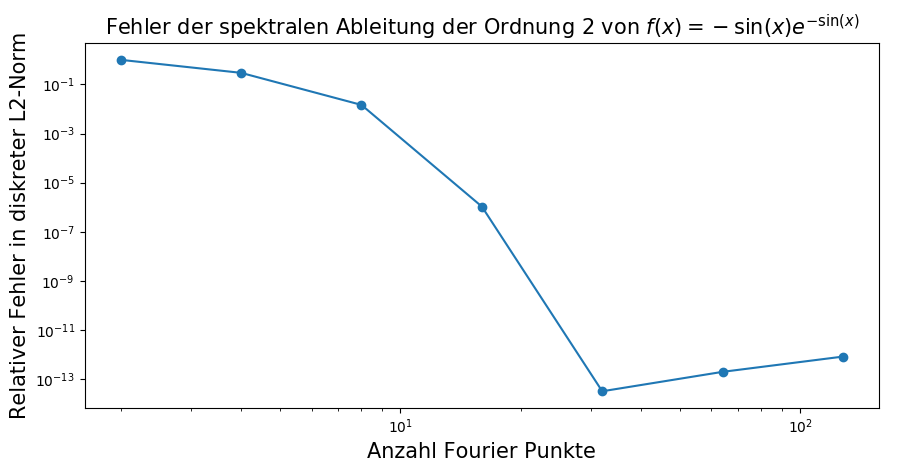
\includegraphics[width=0.9\linewidth]{Figures/spectral_derivative_error_cont.png}
  \caption{Konvergenz der spektralen Ableitung zweiter Ordnung von $f_1$.}
\end{figure}
\begin{figure}[!htb]
  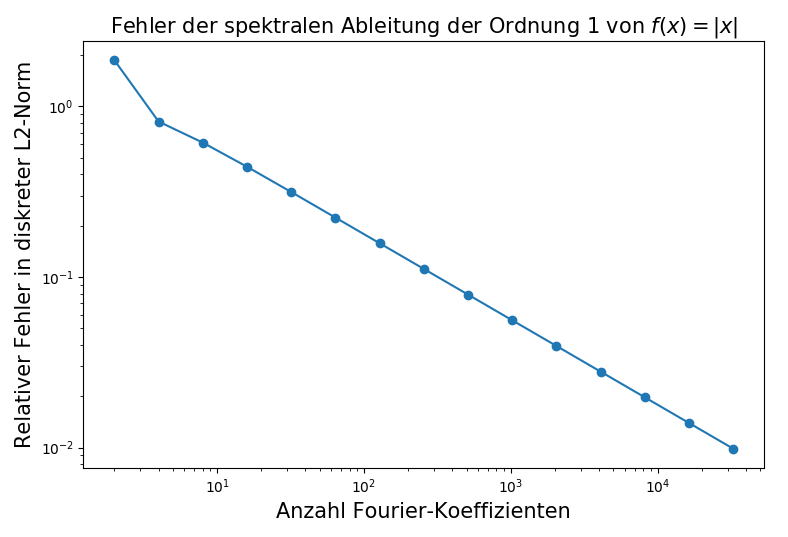
\includegraphics[width=0.9\linewidth]{Figures/spectral_derivative_error_discont.png}
  \caption{Konvergenz der spektralen Ableitung zweiter Ordnung von $f_2$.}
\end{figure}
Wir erkennen, dass die analytische Funktion $f_1$ eine exponentielle Konvergenz aufweist und bereits für $2N=64$ Punkte im Bereich der Maschinengenauigkeit liegt. Rechenfehler sorgen für größeres $N$ für eine Aufsummierung von kleinen Überschwingungen und einen langsam wachsenden Fehler.\\
Die stetige Funktion $f_2$ mit stückweise stetiger nicht-periodischer Ableitung leidet bei der Approximation unter dem Gibbs-Phänomen und deutlich langsamerer Konvergenz.
\end{mathbsp}

Formalisieren wir nun die diskrete Fouriertransformation, die wir verwenden möchten, um eine Approximation an die Fourier-Koeffizienten zu erhalten.
\begin{mathdef}[Diskrete Fourier-Transformation]
Die lineare Abbildung $\mathcal{F}_N\colon\Complex^N\to\Complex^N$ definiert durch
\[\mathcal{F}_Nz=\fourier{z},\qquad\text{mit}\quad \fourier{z}_k=\sum_{j=0}^{N-1}e^{-2\pi i\frac{jk}{N}-ik\pi}z_j\]
heißt diskrete Fourier-Transformation.
\end{mathdef}
Anstelle die direkte Implementierung von $\mathcal{F}_N$ zu verwenden, welche $\mathcal{O}(N^2)$ Rechenschritte benötigt, werden wir auf die deutlich schnellere Berechnung der Abbildung in $\mathcal{O}(N\log N)$ Schritten zurückgreifen, bekannt unter dem Namen \emph{Fast Fourier Transform}(fft). Da diese auf der Annahme $N=2^p$ für ein $p\in\N$ basiert, werden wir in Zukunft nur noch solche Approximationen verwenden. Dies ist essentiell, um eine schnelle Berechnung der Lösung der KGG zu gewährleisten. Ohne Beweis gilt $\mathcal{F}_N\overline{\mathcal{F}}_N=NI$ und somit hat die inverse Fourier-Transformation beinahe die selbe Gestalt wie die Fourier-Transformation selbst und kann ebenso schnell berechnet werden.\\
Im Folgenden nehmen wir an, die Fourier-Approximation (\ref{eqn:fourier_approx}) von $u$ sei exakt und berechnen für den $j$-ten Punkt $x_j$ der Diskretisierung
\begin{equation}
\label{eqn:laplace_approxu}
\Laplace u(t,x_j)=\sum_{k\in\mathcal{I}_N}\fourier{u}_k(t)\Laplace e^{ikx_j}=\sum_{k\in\mathcal{I}_N}-k^2\fourier{u}_k(t)e^{ikx_j}
\end{equation}
Betrachten wir nun $(\Laplace u(t,x_j))_{j=0,\dots,N-1}^T$ für den Vektor $u_N(t)=(u(t,x_j))_{j=0,\dots,N-1}^T$ so gilt
\[(\Laplace u(t,x_j))_{j=0,\dots,N-1}^T\approx \mathcal{F}_N^{-1}\left(\big(-k^2\big)_{k\in\mathcal{I}_N}\odot\mathcal{F}_Nu_N(t)\right)\]
wobei $\odot$ die komponentenweise Multiplikation der Vektoren bezeichnet.\\
Damit erhalten wir für $\beta_N=(\beta(x_j))_{j=0,\dots,N-1}$ die im Ort diskretisierte KGG
\begin{equation}
\label{eqn:kgg_discretespace}
\dtt{u}_N(t)=\alpha \mathcal{F}_N^{-1}\left(\big(-k^2\big)_{k\in\mathcal{I}_N}\odot\mathcal{F}_Nu(t)_N\right) -\beta_N\odot u_N(t)
\end{equation}
Diese werden wir nun in ein System erster Ordnung umschreiben, um anschließend ein Splitting darauf anzuwenden. 

Es gilt für $t>0$, $v_N(t)\coloneqq \dt u_N(t)$ und ein Gewicht $w\in [0,1]$ die zu (\ref{eqn:kgg_discretespace}) äquivalente Darstellung
\begin{align}
\label{eqn:kgg_discrete_first_order_part1}
\dt{\begin{pmatrix}u_N\\v_N\end{pmatrix}}(t)&=
\begin{pmatrix}0 & wI_N\\ \alpha\mathcal{F}_N^{-1}\left(\big(-k^2\big)_{k\in\mathcal{I}_N}\odot\mathcal{F}_N (\cdot )\right) & 0\end{pmatrix}
\begin{pmatrix}u_N\\v_N\end{pmatrix}(t)\\
\label{eqn:kgg_discrete_first_order_part2}
&\quad+\begin{pmatrix}0 & (1-w)I_N\\ -\diag({\beta_N}) & 0\end{pmatrix}
\begin{pmatrix}u_N\\v_N\end{pmatrix}(t)
\end{align}
\subsubsection*{Numerischer Fluss des ersten Teils}
Zuerst betrachten wir den ersten Teil der im Ort diskretisierten KGG (\ref{eqn:kgg_discrete_first_order_part1}) und schreiben diesen für $\fourier{u}_N=\mathcal{F}_Nu_N$ und $\fourier{v}_N=\mathcal{F}_Nv_N$ als
\begin{align*}
\dt{\begin{pmatrix}u_N\\v_N\end{pmatrix}}(t)&=
\begin{pmatrix}0 & wI_N\\ \alpha\mathcal{F}_N^{-1}\left(\big(-k^2\big)_{k\in\mathcal{I}_N}\odot\mathcal{F}_N (\cdot )\right) & 0\end{pmatrix}
\begin{pmatrix}u_N\\v_N\end{pmatrix}(t)\\
\equivalent 
\dt{\begin{pmatrix}\fourier{u}_N\\\fourier{v}_N\end{pmatrix}}(t)&=
\begin{pmatrix}0 & wI_N\\ \alpha\diag\big(-k^2\big)_{k\in\mathcal{I}_N} & 0\end{pmatrix}
\begin{pmatrix}\fourier{u}_N\\\fourier{v}_N\end{pmatrix}(t)
\end{align*}
Damit haben wir nun ein System gewöhnlicher Differentialgleichungen der Größe $2N$ im Fourierraum, welches wir explizit über die Matrixexponentialfunktion lösen können:
\[\begin{pmatrix}\fourier{u}_N\\\fourier{v}_N\end{pmatrix}(t)=\exp\underbrace{\left(t\begin{pmatrix}0 & wI_N\\ \alpha\diag\big(-k^2\big)_{k\in\mathcal{I}_N} & 0\end{pmatrix}\right)}_{=M}
\begin{pmatrix}\fourier{u}_N\\\fourier{v}_N\end{pmatrix}(0)\]
Die Blockmatrix $M$ lässt sich in eine äquivalente Blockdiagonalmatrix umformen, indem zueinander gehörende Einträge der $\fourier{u}_N$ und $\fourier{v}_N$ nebeneinander getauscht werden. Die Matrixexponentialfunktion von $M$ lässt sich dann durch die Matrixexponentialfunktion der $2\times 2$ Blöcke $M_k$ berechnen. 
\[\exp(M_k)=\exp\begin{pmatrix}0 & wt\\ -\alpha k^2t & 0\end{pmatrix}=
\begin{pmatrix}\cos(t\sqrt{\alpha w}|k|) & \sinc(t\sqrt{\alpha w}|k|)tw\\-\sinc(t\sqrt{\alpha w}|k|)\alpha |k|^2t & \cos(t\sqrt{\alpha w}|k|)\end{pmatrix}\]
Wir fassen nun die Ergebnisse zum numerischen Fluss des ersten Teil des Splittings (\ref{eqn:kgg_discrete_first_order_part1}) zusammen.\\
Seien $g$ und $h$ die Anfangswerte, so gilt $\fourier{u}_N(0)=\mathcal{F}_Ng$ und $\fourier{v}_N(0)=\mathcal{F}_Nh$. Die Lösung an den Stellen $x_j=-\pi+2\pi\frac{j}{N}\in [-\pi,\pi)$ für $j=0,\dots,N-1$ lässt sich darstellen als
\begin{align*}
u(t,x_j)&=\left(\mathcal{F}_N^{-1}\left[\mathcal{F}_Ng\odot \big(\cos(t\sqrt{\alpha w}|k|)\big)_{k\in\mathcal{I}_N} + \mathcal{F}_Nh\odot \big(\sinc(t\sqrt{\alpha w}|k|)tw\big)_{k\in\mathcal{I}_N}\right]\right)_j\\
\dt{u}(t,x_j)&=\left(\mathcal{F}_N^{-1}\left[\mathcal{F}_Ng \odot \big(-\sinc(t\sqrt{\alpha w}|k|)\alpha|k|^2t\big)_{k\in\mathcal{I}_N}+\mathcal{F}_Nh\odot \big(\cos(t\sqrt{\alpha w}|k|)\big)_{k\in\mathcal{I}_N}\right]\right)_j
\end{align*}
Man beachte, dass die Sortierung der Fourier-Koeffizienten in verschiedenen Programmiersprachen verschiedenen Notationen folgt und entsprechend die Indizierung angepasst werden muss. Beispielsweise gilt für die Python3 Bibliothek \emph{numpy} durch die entsprechende Funktion \emph{numpy.fft.fftfreq(8)*8} die Konvention
\[\mathcal{I}_8=\left( 0,  1,  2,  3, -4, -3, -2, -1\right)\]
wobei Matlab die ähnliche Konvention
\[\mathcal{I}_8=\left( 0,  1,  2,  3, 4, -3, -2, -1\right)\]
verwendet.\\[0.3cm]
Obige Erläuterungen waren für eine räumliche Dimension $d=1$. Will man nun den Ansatz auf mehrere Dimensionen erweitern, so erhält man ein sehr ähnliches Ergebnis.
Führt man die Fourier-Transformation in jeder Dimension durch, so ergibt sich für $d=2$ die Approximation
\[u(t,x)\approx\sum_{k_1\in\mathcal{I}_N}\fourier{u}_{k_1}(t,x_2)e^{ik_1x_1}=\sum_{k_1\in\mathcal{I}_N}\sum_{k_2\in\mathcal{I}_N}\fourier{u}_{k_1,k_2}(t)e^{i(k_1x_1+k_xx_2)}\]
und analog zu der Approximation (\ref{eqn:laplace_approxu}) erhält man
\[\Laplace u(t,x)=\sum_{k_1\in\mathcal{I}_N}-k_1^2\fourier{u}_{k_1}(t,x_2) e^{ik_1x_1}=\sum_{k_1,k_2\in\mathcal{I}_N}-(k_1^2+k_2^2)\fourier{u}_{k_1,k_2}(t)e^{i(k_1x_1+k_2x_2)}\]
Das Vorgehen im mehrdimensionalen unterscheidet sich also nur durch eine aufwändigere Indizierung, ist jedoch im Kern dieselbe. Ersetzt man in obigen Ausführungen für $d=1$ sämtliche $|k|$ durch \[\norm{k}_2=\sqrt{k_1^2+\dots+k_d^2}\]so erhält man, bei passender Indizierung der diskreten Fourier-Approximation, eine Darstellung der Lösung für beliebige Dimensionen $d\in\N$.
\subsubsection*{Method of lines für zweiten Teil des Splittings}
Einen Löser für den zweiten Teil (\ref{eqn:kgg_discrete_first_order_part1}) der im Ort diskretisierten KGG erhält man auf ähnliche Weise. Wir suchen für $t>0$, $\beta(x)>0$ und ein Gewicht $\tilde{w}=1-w\in [0,1]$ die Lösung der Differentialgleichung
\begin{equation*}
\dt{\begin{pmatrix}u_N\\v_N\end{pmatrix}}(t)=
\begin{pmatrix}0 & \tilde{w}I_N\\ -\diag({\beta_N}) & 0\end{pmatrix}
\begin{pmatrix}u_N\\v_N\end{pmatrix}(t)
\end{equation*}
Wiederum lässt sich die Lösung der Differentialgleichung mithilfe der Matrixexponentialfunktion darstellen. Die Matrixexponentialfunktion der Blockmatrix wiederum ist äquivalent zu einer umsortierten Blockdiagonalmatrix für welche gilt
\[\exp\begin{pmatrix}0 & \tilde{w}t\\ -t\beta(x_j) & 0\end{pmatrix}=
\begin{pmatrix}\cos(t\sqrt{\beta(x_j)\tilde{w}}) & \sinc(t\sqrt{\beta(x_j)\tilde{w}})\tilde{w}t\\
-\sinc(t\sqrt{\beta(x_j)\tilde{w}})\beta(x_j)t & \cos(t\sqrt{\beta(x_j)\tilde{w}})\end{pmatrix}\]
Daraus erhalten wir also zu den Anfangswerten $g$ und $h$ für festes $x\in \Torus^d$ die explizite Lösung des zweiten Teil des Splittings durch
\[\begin{pmatrix}u\\v\end{pmatrix}(t,x)=
\begin{pmatrix}\cos(t\sqrt{\beta(x)\tilde{w}}) & \sinc(t\sqrt{\beta(x)\tilde{w}})\tilde{w}t\\
-\sinc(t\sqrt{\beta(x)\tilde{w}})\beta(x)t & \cos(t\sqrt{\beta(x)\tilde{w}})\end{pmatrix}
\begin{pmatrix}g\\h\end{pmatrix}(x)\]
Wir benötigen im Gegensatz zum ersten Teil keine feste Ortsdiskretisierung und bekommen sogar eine exakte Lösung des Teilproblems. Da die Punkte für die verschiedenen Teile des Splittings zusammen passen müssen, sind wir jedoch durch die Anforderung festgelegt, die die Fourierapproximation an die Punkte stellt.\\
Mithilfe der \emph{method of lines}, d.h. punktweiser Auswertung der Lösung für alle benötigten $x$, bekommt man schlussendlich eine numerische Lösung.
\subsubsection*{Konkretisierung des Algorithmus}
Wir haben nun also zwei separate Einschrittverfahren, die zusammen mit dem Strang-Splitting Framework einen guten Löser für die KGG ergeben. Dieses Lösungsverfahren ist für $d=1$ schematisch als Algorithmus \ref{alg:kgg_solver} dargestellt.
\begin{algorithm}[ht]
    \caption{Strang-Splitting für KGG}
    \label{alg:kgg_solver}
    \begin{algorithmic}[1] % The number tells where the line numbering should start
        \Function{Strang\_Step\_KGG}{$N,u_0,v_0,\alpha,\beta,w,\tau$} 
            \State $x_N\gets (-\pi+\frac{2\pi j}{N})_{j=0,\dots,N-1}^T$
            \State $g,h\gets u_0(x_N), v_0(x_N)$
            \State $g,h\gets \text{First\_Part\_Solver}(N, g, h, \alpha, w, \frac{\tau}{2})$
            \State $g,h\gets \text{Second\_Part\_Solver}(x_N, g, h, \beta, 1-w, \tau)$
            \State $u_1,v_1\gets \text{First\_Part\_Solver}(N, g, h, \alpha, w, \frac{\tau}{2})$
            \State \textbf{return} $u_1, v_1$\Comment{Approximation an $u(\tau,x_N)$ und $\dt{u}(\tau,x_N)$}
        \EndFunction
        
        \Function{First\_Part\_Solver}{$N,g,h,\alpha,w,\tau$} 
        	\State Indexmenge $\mathcal{I}_N$ für Fourierkoeffizienten initialisieren
        	\State $\fourier{g}\gets \mathcal{F}_Ng$
        	\State $\fourier{h}\gets \mathcal{F}_Nh$
        	\State $c\gets \big(\cos(\tau\sqrt{\alpha w}|k|)\big)_{k\in\mathcal{I}_N}$
        	\State $s_1\gets \big(\sinc(\tau\sqrt{\alpha w}|k|)\tau w\big)_{k\in\mathcal{I}_N}$
        	\State $s_2\gets \big(-\sinc(\tau\sqrt{\alpha w}|k|)\alpha|k|^2\tau\big)_{k\in\mathcal{I}_N}$
            \State \textbf{return} $\mathcal{F}_N^{-1}\left(\fourier{g}\odot c+\fourier{h}\odot s_1\right),\quad \mathcal{F}_N^{-1}\left(\fourier{g}\odot s_2+\fourier{h}\odot c\right)$
        \EndFunction
        \Function{Second\_Part\_Solver}{$x_N,g,h,\beta,\tilde{w},\tau$} 
        	\State $\beta_N\gets\beta(x_N)$
        	\State $c\gets \cos(\tau\sqrt{\beta_N}\sqrt{\tilde{w}})$
        	\State $s_1\gets \sinc(\tau\sqrt{\beta_N}\sqrt{\tilde{w}})\tilde{w}\tau$
        	\State $s_2\gets -\sinc(\tau\sqrt{\beta_N}\sqrt{\tilde{w}})\beta_N\tau$
        	\State \textbf{return} $g\odot c+h\odot s_1,\quad g\odot s_2+h\odot c$
        \EndFunction
    \end{algorithmic}
\end{algorithm}

Dabei ist die Wahl gewisser Parameter jedoch noch unklar:
\begin{itemize}
\item Die Anzahl der Fourierpunkte $N$.
\item Das Gewicht $w\in[0,1]$ für die Gewichtung des Splittings. 
\end{itemize}
Um die Zusammenhänge und Probleme besser zu verstehen, werden wir anhand eines Beispiels mit bekannter exakter Lösung verschiedene Kombinationen der Parameter demonstrieren.
\begin{mathbsp}
\label{bsp:trialfrog2}
Seien $c>2$ und $d\neq 0$, dann ist
\begin{align*}
u(t,x)&=\frac{\cos(dt)}{\sin(x)+c}\\
u_0(x)&=\frac{1}{\sin(x)+c}\\
v_0(x)&\equiv 0\\
\end{align*}
eine Lösung der KGG (\ref{kgg}) mit $\alpha=c-2$ und $\beta(x)=d^2+(c-2)\left(\frac{\sin(x)}{\sin(x)+c}+\frac{2\cos^2(x)}{(\sin(x)+c)^2}\right)$. Wir lösen nun die KGG mithilfe verschiedener Splitting Varianten und beobachten in Abbildung \ref{fig:splitting_convergence}
\begin{itemize}
\item für das Strang-Splitting die erwartete Konvergenz von Ordnung 2.
\item für das Lie-Trotter-Splitting die erwartete Konvergenz von Ordnung 1.
\item für die schnelle Variante des Strang-Splittings (FastStrang), bei der die äußeren Halbschritte kombiniert werden, exakt den gleichen Fehler wie beim normale Strang-Splitting.
\item für die umgekehrte Variante des Strang-Splittings (ReversedStrang), wo die Reihenfolge der beiden Aufteilungen der Gleichung vertauscht wurde, eine minimale Abweichung von der normalen Variante.
\item ein deutliches Problem: Wird die Zeitschrittweite $\tau$ zu groß, d.h. ist $1.227\tau>\frac{2\pi}{N}=h$, so ist das Verfahren instabil!
\end{itemize}
\begin{figure}[!htb]
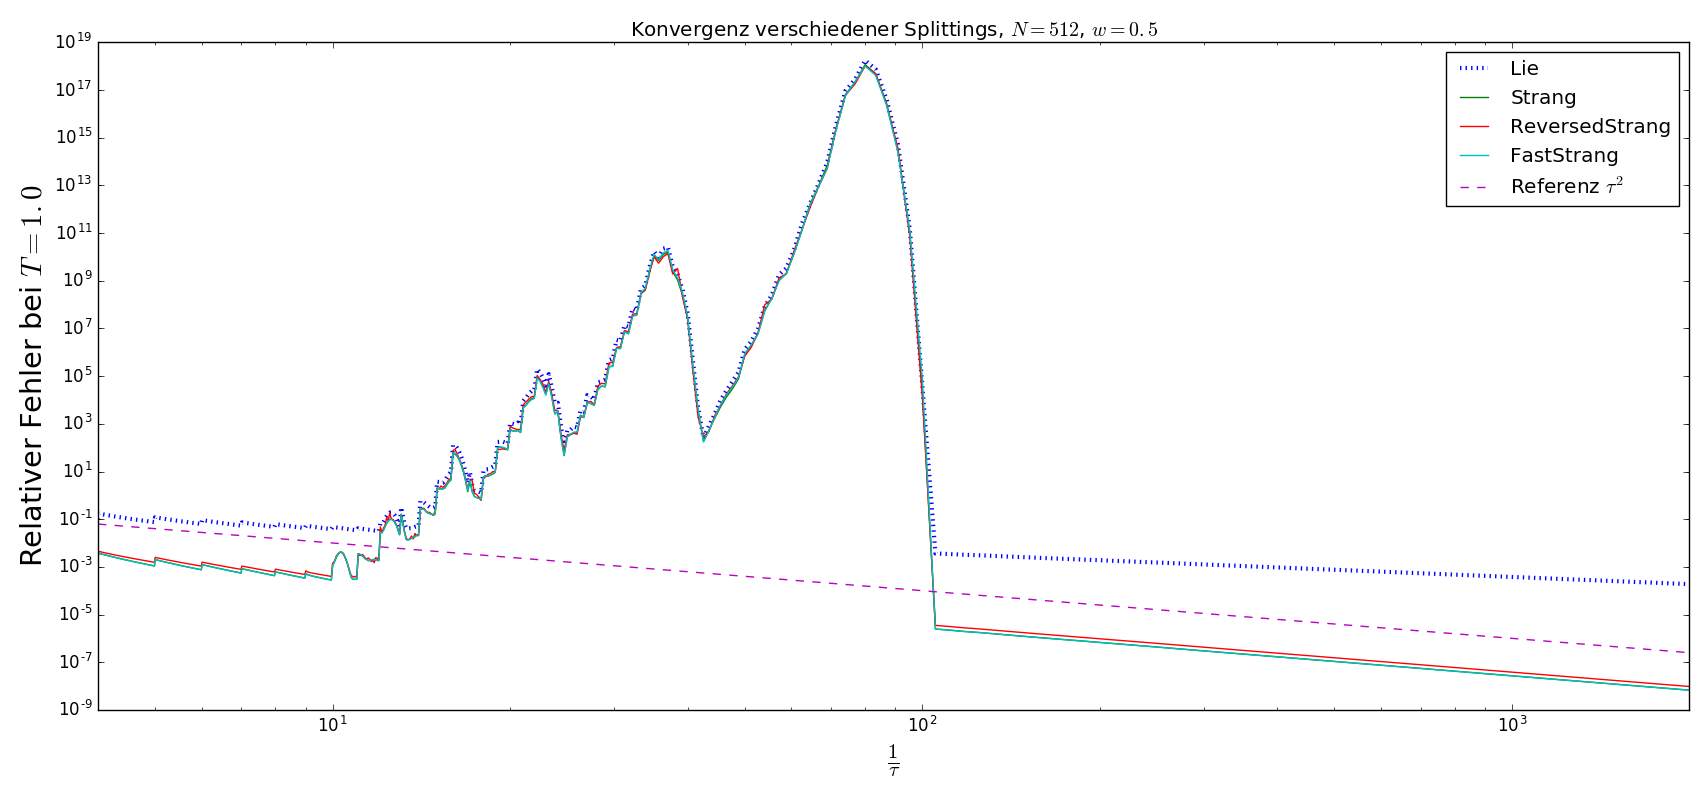
\includegraphics[width=\textwidth]{Figures/splitting_convergence_fix_weight_frog2_cfl.png}
\caption{Konvergenzordnung für verschiedene Splitting Varianten anhand von Beispiel \ref{bsp:trialfrog2} mit $c=3$, $d=1$, $N=512$, $w=0.5$ zum Zeitpunkt $T=1$.}
\label{fig:splitting_convergence}
\end{figure}
Für die beobachtete Instabilität spielt der Gewichtsfaktor $w$ eine große Rolle. Wäre $w=0$, so entspricht der Löser des ersten Teil des Splittings der Vorschrift
\begin{align*}
u(t,x_N)&=\mathcal{F}_N^{-1}\left(\mathcal{F}_Ng(x_N)\right)=g(x_N)=u(0,x_N)\\
\dt{u}(t,x_N)&=\mathcal{F}_N^{-1}\left(\mathcal{F}_Ng(x_N)\odot \big(-\alpha |k|^2t\big)_{k\in\mathcal{I}_N}\right)+h(x_N)\\
&=t \alpha \mathcal{F}_N^{-1}\left(\mathcal{F}_N\odot \big(-|k|^2\big)_{k\in\mathcal{I}_N}\right)+h(x_N)\\
&=t\alpha \Laplace_N g(x_N)+h(x_N)\\
&\approx t\dtt{u}(0,x_N)+\dt{u}(0,x_N)
\end{align*}
Somit wird in diesem Randfall nur die erste Ableitung geändert und dieses Update entspricht einem expliziten Eulerschritt. Wir erhalten eine \emph{Courant-Friedrichs-Lewy-Bedingung} (CFL-Bedingung) der Form $\tilde{c}\tau\le h=\frac{2\pi}{N}$. Im Fall $k=0$ entspricht die CFL-Zahl $\tilde{c}$ der CFL-Zahl des expliziten Eulers. Andernfalls beobachten wir, dass die CFL-Zahl abhängig von $w$ ist und für $w=1$ ein Minimum annimmt. Wie man an Abbildung \ref{fig:splitting_convergence_w1} erkennt, verhält sich für $w=1$ die Gleichung am stabilsten und kann auch für große Zeitschrittweiten sinnvoll gelöst werden. Dies wird eine große Motivation dafür sein, das Gewicht $w=1$ zu wählen.

\begin{figure}[!htb]
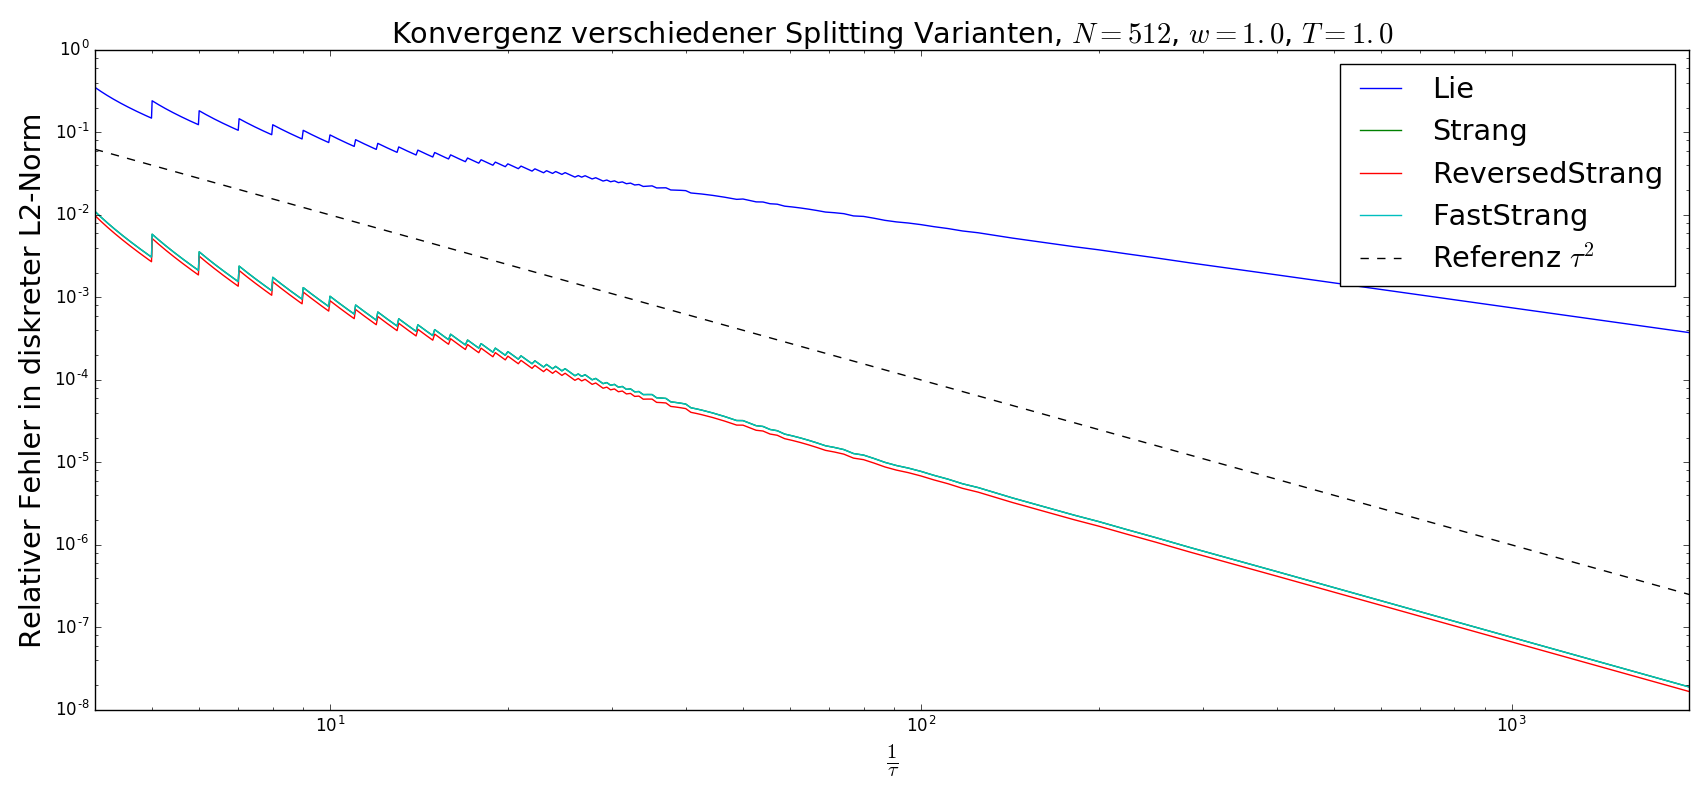
\includegraphics[width=\textwidth]{Figures/splitting_convergence_fix_weight_frog2_cfl_corrected.png}
\caption{Konvergenzordnung für verschiedene Splitting Varianten anhand von Beispiel \ref{bsp:trialfrog2} mit $c=3$, $d=1$, $N=512$, $w=1$ zum Zeitpunkt $T=1$.}
\label{fig:splitting_convergence_w1}
\end{figure}
Zuletzt sei aber erwähnt, dass die Wahl $w=1$ aus Sicht des minimalen Fehlers selten optimal ist. An Abbildung \ref{fig:splitting_dependence_on_weight} erkennen wir für verschiedene bekannte Lösungen der KGG, dass das Minimum des Fehlers in Abhängigkeit vom Gewicht $w$ sowohl an beiden Rändern, als auch als lokales Minimum auftreten kann. Das genaue Minimum zu bestimmen und dies mit der CFL-Zahl zu kombinieren, um das optimale $w$ zu wählen, kann ein möglicher Ansatz zur Verbesserung des Algorithmus sein. Wir werden dies jedoch nicht weiter verfolgen und uns auf $w=1$ beschränken, da eine Verbesserung des Fehlers dann mit einer Verringerung der Schrittweite $\tau$ immer möglich ist.
\begin{figure}[!htb]
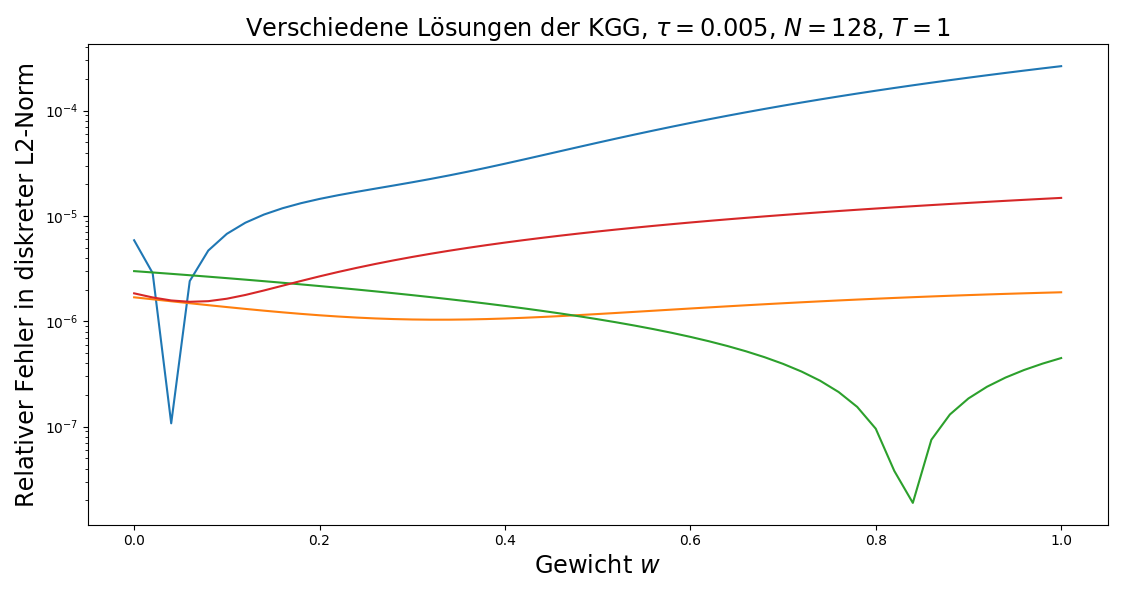
\includegraphics[width=\textwidth]{Figures/splitting_error_over_weights.png}
\caption{Verschiedene Beispiele von bekannten Lösungen der KGG gelöst mit FastStrang. Der Fehler wird dabei in Abhängigkeit des Gewichts $w$ verglichen.}
\label{fig:splitting_dependence_on_weight}
\end{figure}
\end{mathbsp}
\section{Polynome und Verteilungen}
Die Theorie des general Polynomial Chaos ist die Grundlage für später vorgestellte Verfahren zum Lösen von der stochastischen Klein-Gordon-Gleichung. Im Mittelpunkt dieser Theorie stehen orthogonale Polynombasen. Die Verflechtung mit der Stochastik geschieht dann auf natürliche Weise durch die passende Wahl des zugrunde liegenden Skalarproduktes.
\subsection{Orthogonale Polynome}
Wir beginnen mit grundlegender Notation und Namensgebung um das zentrale Werkzeug der Polynomapproximation festzulegen. Später werden diese Polynome verwendet, um die Zufallsabhängigkeit der auftretenden Funktionen darzustellen, indem das Orthogonalitätsmaß der Dichtefunktion entspricht.
\begin{mathdef}
Ein allgemeines Polynom $Q$ vom Grad $n$ lässt sich darstellen als
\[Q_n(x)=q_nx^n+q_{n-1}^{n-1}+\dots+q_1x+q_0,\quad q_n\ne 0\]
Wir bezeichnen mit 
\[\frac{Q_n(x)}{q_n}\]
die normierte (engl. \emph{monic}) Version des Polynoms $Q$, also mit führendem Koeffizienten gleich 1.\\
 Ein System $\left\lbrace Q_n(x),\: n\in\mathcal{N}\right\rbrace$ von Polynomen mit $\mathcal{N}=\N_0=\N\cup\lbrace 0\rbrace$ oder $\mathcal{N}=\lbrace 0,1,\dots,N-1,N\rbrace$ heißt Orthogonalsystem, wenn bezüglich eines reellen positiven Maßes $\alpha$ die Orthogonalitätsbedingung
 \[\langle Q_n(x),Q_m(x)\rangle =\int_S Q_n(x)Q_m(x)d\alpha(x)=\gamma_n\delta_{mn},\quad m,n\in\mathcal{N}\]
 erfüllt ist. Dabei ist $\delta_{mn}$ das Kronecker-Delta, $S$ der nicht notwendigerweise endliche Träger des Maßes $\alpha$ und $y_n>0$ die Normalisierungskonstanten. Es gilt 
 \[\gamma_n=\int_S Q_n^2(x)d\alpha(x),\quad n\in\mathcal{N}\] und O.B.d.A. werden wir in folgenden Kapiteln stets von $\gamma_n=1$ ausgehen. In diesem Fall nennt man das System ein Orthonormalsystem.
\end{mathdef}
Das Hermite Chaos ist ein motivierendes Beispiel dafür, dass solche Verflechtungen von Polynombasis und stochastischer Verteilung natürlicherweise existieren.
\begin{mathbsp}[Hermite Chaos]
Ist $S=(-\infty,\infty)$, $w(x)=\frac{1}{\sqrt{2\pi}}e^{-\frac{x^2}{2}}$ die Dichtefunktion des Gauss-Verteilung und verwenden wir diese als Dichte des Maßes $\alpha$, so sind die Hermite Polynome
\[H_0(x)\equiv 1,\quad H_1(x)=x,\quad H_2(x)=x^2-1,\quad H_n(x)=xH_{n-1}(x)-(n-1)H_{n-2}(x)\]
ein Orthogonalsystem bezüglich $\langle\cdot,\cdot\rangle_{L_w^2(S)}$ mit Normalisierungskonstanten $\gamma_n=n!$.\\
Der Erwartungswert der Gauss-Verteilung
\[\E_w[Z]= \int_{-\infty}^\infty Z(x)w(x)dx\] erfüllt also die entscheidende Beziehung des Polynomial Chaos
\[\langle H_n,H_m\rangle_{L_w^2(S)} =\E_w \left[H_nH_m\right]=\gamma_n\delta_{nm}\]
Man beachte, dass diese Definition der Hermite Polynome leicht von der in der Literatur üblichen abweicht. Dies ist der Tatsache geschuldet, dass dort die entsprechende Gewichtsfunktion einen zusätzlichen Faktor $\sqrt{2}$ besitzt. Sie stellt somit keine Dichte einer Wahrscheinlichkeitsverteilung dar und ist für unsere Zwecke unpraktisch und wird nicht verwendet. 
\end{mathbsp}
Wir werden in dieser Arbeit auf Polynombasen, die diskreten Verteilungen entsprechen, verzichten. Es sei jedoch bemerkt, dass dies keine Einschränkung der Methode ist, sondern lediglich die Notation vereinfacht. Konkret werden wir uns mit Laguerre-, Jacobi-, Hermite- und Legendre-Polynomen beschäftigen, wobei letztere ein Spezialfall der Jacobipolynome darstellen. Details und Eigenschaften sind im Anhang \ref{AppendixA} zu finden.\\[0.3cm]
Eine wichtige Eigenschaft von Orthogonalsystemen von Polynomen ist eine besondere Art der rekursiven Darstellung, wie wir sie bereits bei den Hermite Polynomen gesehen haben.
\begin{maththeorem}[Drei Term Rekursion]
\label{threetermexist}
Ein Orthogonalsystem $\left\lbrace Q_n(x),\: n\in\N_0\right\rbrace$ von Polynomen erfüllt eine Drei-Term-Rekursion
\begin{eqnarray}
Q_n(x)=(a_nx+b_n)Q_{n-1}(x)-c_nQ_{n-2}(x),\quad n\in\N\\
Q_{-1}(x)\equiv 0, Q_0(x)\equiv 1\nonumber
\end{eqnarray}
wobei $a_n=\frac{k_n}{k_{n-1}}\neq 0$, $b_n\in\R$ und $c_n=\frac{a_n}{a_{n-1}}\cdot \frac{\gamma_n}{\gamma_{n-1}}$.
Dabei ist $k_n\neq 0$ der führende Faktor und $\gamma_n>0$ der Normalisierungsfaktor des Polynoms $Q_n$ . 
\end{maththeorem}
\begin{proof}
Es gilt $\text{deg}(Q_n)=n,\forall n\in\N_0$. Für $a_n=\frac{k_n}{k_{n-1}}$ ist $Q_n(x)-a_nxQ_{n-1}(x)$ ein Polynom vom Grad $\le n-1$. Dieses lässt sich also schreiben als
\[Q_n(x)-a_nxQ_{n-1}(x)=\sum_{m=0}^{n-1}r_mQ_m(x)\]
Für $k\le n-1$ folgt also aus der Orthogonalität bezüglich des Skalarproduktes $\langle\cdot,\cdot\rangle$
\begin{equation*}
\langle Q_n(x)-a_nxQ_{n-1}(x),Q_k(x)\rangle=\sum_{m=0}^{n-1}r_m\langle Q_m(x),Q_k(x)\rangle=r_k\langle Q_k(x),Q_k(x)\rangle=r_k\gamma_k
\end{equation*}
und durch Verwenden von $\langle Q_n(x),Q_k(x)\rangle = 0$ und Umstellen
\[ -a_n\langle Q_{n-1}(x),xQ_k(x)\rangle=r_k\gamma_k\]
Somit folgt für $k<n-2$ wegen $\text{deg}(xQ_k(x))<n-1$ dass $r_k=0$. Damit erfüllen die Polynome eine Drei-Term-Rekursion
\[Q_n(x)-a_nxQ_{n-1}(x)=r_{n-1}Q_{n-1}(x)+r_{n-2}Q_{n-2}(x)\]
Nun definieren wir $b_n=r_{n-1}$, $c_n=-r_{n-2}$ und berechnen schlussendlich
\[r_{n-2}\gamma_{n-2}=\langle -a_nxQ_{n-1}(x),Q_{n-2}(x)\rangle =-a_n\langle Q_{n-1}(x),xQ_{n-2}(x)\rangle=-a_n\frac{k_{n-2}}{k_{n-1}}\gamma_{n-1}\]
\end{proof}
Diese und noch viele weitere Eigenschaften von den verschiedenen Orthogonalsystemen von Polynomen finden sich in \autocite{weborthopoly} und in vielen weiteren Werken über Polynome. Beispielsweise lässt sich auch die Umkehrung zeigen (unter milden Anforderungen an die Koeffizienten): Zu jeder durch eine Drei-Term-Rekursion definierte Menge an Polynomen existiert ein Maß $\alpha$, bezüglich dessen die Polynome ein Orthogonalsystem bilden (Satz von Favard).\\[0.3cm]
Die auftretenden Integrale in den Skalarprodukten werden wir später mit Gauss-Quadraturformeln approximieren. Unter anderem dafür werden wir später die Nullstellen der Polynome als Stützstellen benötigen. Basierend auf den Koeffizienten der Drei-Term-Rekursion entwickelten Golub und Welsch in \autocite{GolubWelsch} einen effizienten stabilen Algorithmus, der für die Berechnung der Nullstellen mit der Berechnung der Eigenwerte einer symmetrischen Tridiagonalmatrix auskommt.

\begin{maththeorem}[Golub Welsch Algorithmus]
\label{golubwelschalg}
Ist $\left\lbrace Q_i(x),\: i=0,\dots,n\right\rbrace$ ein Orthogonalsystem von Polynomen welches die Drei-Term-Rekursion
\begin{eqnarray}
\label{threetermgolub}
Q_i(x)=(a_ix+b_i)Q_{i-1}(x)-c_iQ_{i-2}(x),\quad i=1,\dots , n\\
Q_{-1}(x)\equiv 0, Q_0(x)\equiv 1\nonumber
\end{eqnarray}
erfüllt für $a_i>0,c_i>0$, so gilt:
\begin{align*}
Q_n(x_j)=0\: \equivalent \: &x_j\text{ ist Eigenwert von }J=\begin{pmatrix}
\alpha_1 & \beta_1 &  &  &  \\ 
\beta_1 & \alpha_2 & \beta_2 & & \text{\huge0} \\ 
 & \beta_2 & \ddots & \ddots &  \\ 
 &  & \ddots & & \beta_{n-1} \\
\text{\huge0} &  &  & \beta_{n-1} & \alpha_n
\end{pmatrix},\quad j=1,\dots,n\\
&\text{ mit } \alpha_i=-\frac{b_i}{a_i},\quad \beta_i=\sqrt{\frac{c_{i+1}}{a_ia_{i+1}}},\quad i=1,\dots,n
\end{align*}
Die Eigenwerte der symmetrischen Tridiagonalmatrix sind reell und lassen sich mit spezialisierten Algorithmen effizient berechnen. Insbesondere sind alle Nullstellen des Polynoms $Q_n$ reell.
\end{maththeorem}
\begin{proof}
Zuerst schreiben wir die Rekursionen (\ref{threetermgolub}) für $i=1,\dots,n$ in Matrixform und teilen zeilenweise durch $a_i$ und sortieren den Term $xQ_{i-1}$ auf die linke Seite
\begin{equation*}
x\cdot
\underbrace{\begin{pmatrix}Q_0(x)\\ Q_1(x) \\ \vdots \\ \\ \vdots \\ Q_{n-1}(x)\end{pmatrix}}_{=Q(x)}
=\underbrace{\begin{pmatrix}
-\frac{b_1}{a_1} & \frac{1}{a_1} &  &  &  \\ 
\frac{c_2}{a_2} & -\frac{b_2}{a_2} & \frac{1}{a_2} & & \text{\huge0} \\ 
 & \frac{c_3}{a_3} & \ddots & \ddots &  \\ 
 &  & \ddots & & \frac{1}{a_{n-1}} \\
\text{\huge0} &  &  & \frac{c_n}{a_n} & -\frac{b_n}{a_n}
\end{pmatrix}}_{=T}
\begin{pmatrix}Q_0(x)\\ Q_1(x) \\ \vdots \\ \\ \vdots \\ Q_{n-1}(x)\end{pmatrix} 
+\begin{pmatrix}0 \\ 0 \\ \vdots \\ \vdots \\ 0 \\ \frac{Q_{n}(x)}{a_n}\end{pmatrix} 
\end{equation*}
In kompakter Form lässt sich dies darstellen als
\[xQ(x)=TQ(x)+\frac{1}{a_n}Q_n(x)e_n\]
wobei $e_n=(0,\dots,0,1)^T$ der n-te Einheitsvektor ist. Hieran erkennt man sofort, dass $Q_n(x_j)=0\equivalent x_j\text{ ist Eigenwert von }T$.\\
Weiterhin erhalten wir aus Satz \ref{threetermexist}, dass $\frac{c_i}{a_i}=\frac{1}{a_{i-1}}\frac{\gamma_i}{\gamma_{i-1}}$ und somit wäre $T=J$ bereits symmetrisch, wenn die $Q_i$ eine Orthonormalbasis bilden.\\
Andernfalls führen wir eine Äquivalenztransformation durch mit der Diagonalmatrix $D=\text{diag}\left((d_1,\dots,d_n)^T\right)$, so dass $J=DTD^{-1}$. Koeffizientenvergleich ergibt die Bedingung $d_{i+1}=d_i\sqrt{\frac{a_{i+1}}{c_{i+1}a_i}}$; mit einer möglichen Wahl $d_1=1$ des freien Parameters $d_1$ erhalten wir somit die gewünschte symmetrische Matrix.
\end{proof}
Wir bemerken zusätzlich ohne Beweis, dass das Polynom $Q_n$ für $n\ge 1$ insgesamt $n$ verschiedene reelle Nullstellen besitzt. Dies ist eine fundamentale Aussage über Orthogonalpolynome und lässt sich induktiv einsehen unter Ausnutzung von $n$ Vorzeichenwechseln, die durch die Orthogonalität vorhanden sein müssen.

\subsection{Polynomiale Approximationstheorie}
Es gibt sehr viele Ergebnisse über die Approximation von Funktionen $f\colon \R\to\R$ durch Polynome $p\in\Poly_n$. Um ein Gefühl für die Mächtigkeit --aber auch für die Grenzen-- von polynomialer Approximation zu bekommen, werden an dieser Stelle einige zentrale Sätze genannt. Auf Beweise werden wir größtenteils verzichten, jedoch basierend auf \autocite{Trefethen} eine Diskussion der Interpretation dieser Ergebnisse aus dem numerischen Blickwinkel der Interpolation und Quadratur geben.
\begin{maththeorem}[Weierstrass]
Ist $I$ ein beschränktes Intervall und $f\in C^0(\bar{I})$ stetig, dann gibt es für jedes $\epsilon >0$ ein $n\in\N$ und $p\in\Poly_n$, so dass
\[|f(x)-p(x)|<\epsilon,\quad \forall x\in\bar{I}\]
\end{maththeorem}
Folglich gilt für die \emph{gleichmäßige Bestapproximation} $\phi_n$, welche zu $f\in C^0(\bar{I})$ eine eindeutige Lösung $\phi_n(f)\in\Poly_n$ mit minimaler Maximumsnorm ergibt, die Aussage
\[\lim\limits_{n\to\infty}\norm{f-\phi_n(f)}_\infty=0\] 
Dieses Ergebnis sieht sehr vielversprechend aus, jedoch wurde von Faber in \autocite{faber14} gezeigt, dass es kein Interpolationsschema gibt, das für alle stetigen Funktionen auf diese Weise konvergiert. Doch dieser vermeintliche Rückschlag ist in der Praxis selten von Bedeutung! Problematisch sind Interpolationsschemata, die beispielsweise auf gleichverteilten Knotenpunkten basieren und dann unter dem Runge-Phänomen leiden, welches bei Funktionen wie $f(x)=\frac{1}{1+x^2}$ an den Rändern für eine schlechte Approximationsgüte sorgt. Erfüllt $f$ jedoch minimale Glattheitsanforderungen (wie bereits Lipschitzstetigkeit) und verwendet man Chebyshev Interpolationspunkte, so ist die Approximationsgüte bereits bereits für kleines $n$ gesichert.\\[0.3cm]
Im Folgenden lösen wir uns von dem beschränkten Intervall $I$ und lassen auch $I=\R$ oder $I=[0,\infty)$ zu. Außerdem wird die Bestapproximation bezüglich der Maximumsnorm später von wenig Nutzen sein. Daher führen wir zuerst einen neuen normierten Raum ein:
\begin{mathdef}
Sei $w\colon I\to\R_{>0}$ ein Gewicht, dann definieren wir den gewichteten $L^2$ Raum als
\begin{equation*}
L_w^2(I)\coloneqq \left\lbrace v\colon I\to\R | \int_Iv^2(x)w(x)dx<\infty\right\rbrace
\end{equation*}
mit dem inneren Produkt 
\[\langle u,v\rangle_{L_w^2(I)}=\int_I u(x)v(x)w(x)dx,\quad u,v\in L_w^2(I)\]
und zugehöriger Norm
\[\norm{u}_{L_w^2(I)}=\left(\int_I u^2(x)w(x)dx\right)^{\onehalf}\]
\end{mathdef}
Der Begriff der Bestapproximation lässt sich auch auf diesen neuen Raum erweitern. Dazu verwenden wir eine orthogonale Projektion auf eine orthogonale Polynombasis und erhalten eine einfache Darstellung des Bestapproximationsoperators.
\begin{maththeorem}
Ist $N\in\N_0$ und $\lbrace Q_k(x)\rbrace_{k=0}^N\subset \Poly_N$ ein Orthogonalsystem bezüglich des positiven Gewichtes $w(\cdot)$, also 
\[\langle Q_m(x),Q_n(x)\rangle_{L_w^2(I)}=\norm{Q_m}^2_{L_w^2(I)}\delta_{m,n},\quad, 0\le m,n\le N\]
so gilt für den Projektionsoperator $P_N\colon L_w^2(I)\to \Poly_N$ definiert durch 
\[P_Nf\coloneqq \sum_{k=0}^N\hat{f}_kQ_k(x),\quad \hat{f}_k\coloneqq \frac{1}{\norm{Q_k}_{L_w^2(I)}^2}\langle f,Q_k\rangle_{L_w^2(I)},\qquad f\in L^2_w(I),\]
die Bestapproximationsaussage
\[\norm{f-P_Nf}_{L_w^2(I)}=\inf\limits_{\psi\in\Poly_N}\norm{f-\psi}_{L_w^2(I)}\]
\end{maththeorem}
Dies entspricht der Fourier-Entwicklung im Hilbertraum. Entsprechend nennt man die Koeffizienten $\hat{f}_k$ die (verallgemeinerten) Fourier-Koeffizienten. Die Projektion ist eine Orthogonalprojektion in dem Sinne, dass der Fehler $f-P_Nf$ senkrecht zum Polynomraum $\Poly_N$ ist.\\
Man beachte, dass der Name "`Bestapproximation"' sich strikt auf die verwendete Norm bezieht. Punktweise Aussagen lassen sich somit im Allgemeinen nicht treffen. 
\begin{mathbsp}
Als Beispiel vergleichen wir die Bestapproximation bezüglich der Maximumsnorm und die Chebyshev Interpolation vom Grad $N=100$ von der Funktion $f(x)=|x-\frac{1}{4}|$ in $[-1,1]$. Wie wir an Abbildung \ref{polyapproxcomp} erkennen, ist der maximale Fehler der Bestapproximation zwar geringer, aber tritt an $N+2$ Punkten auf, wohingegen der Fehler der Chebyshev Fehler zu den Rändern hin stark abnimmt. Dies soll verdeutlichen, dass die Bestapproximation nicht immer in jedem Sinne die "`beste"' Approximation darstellt.
\begin{figure}[ht]
 \center
 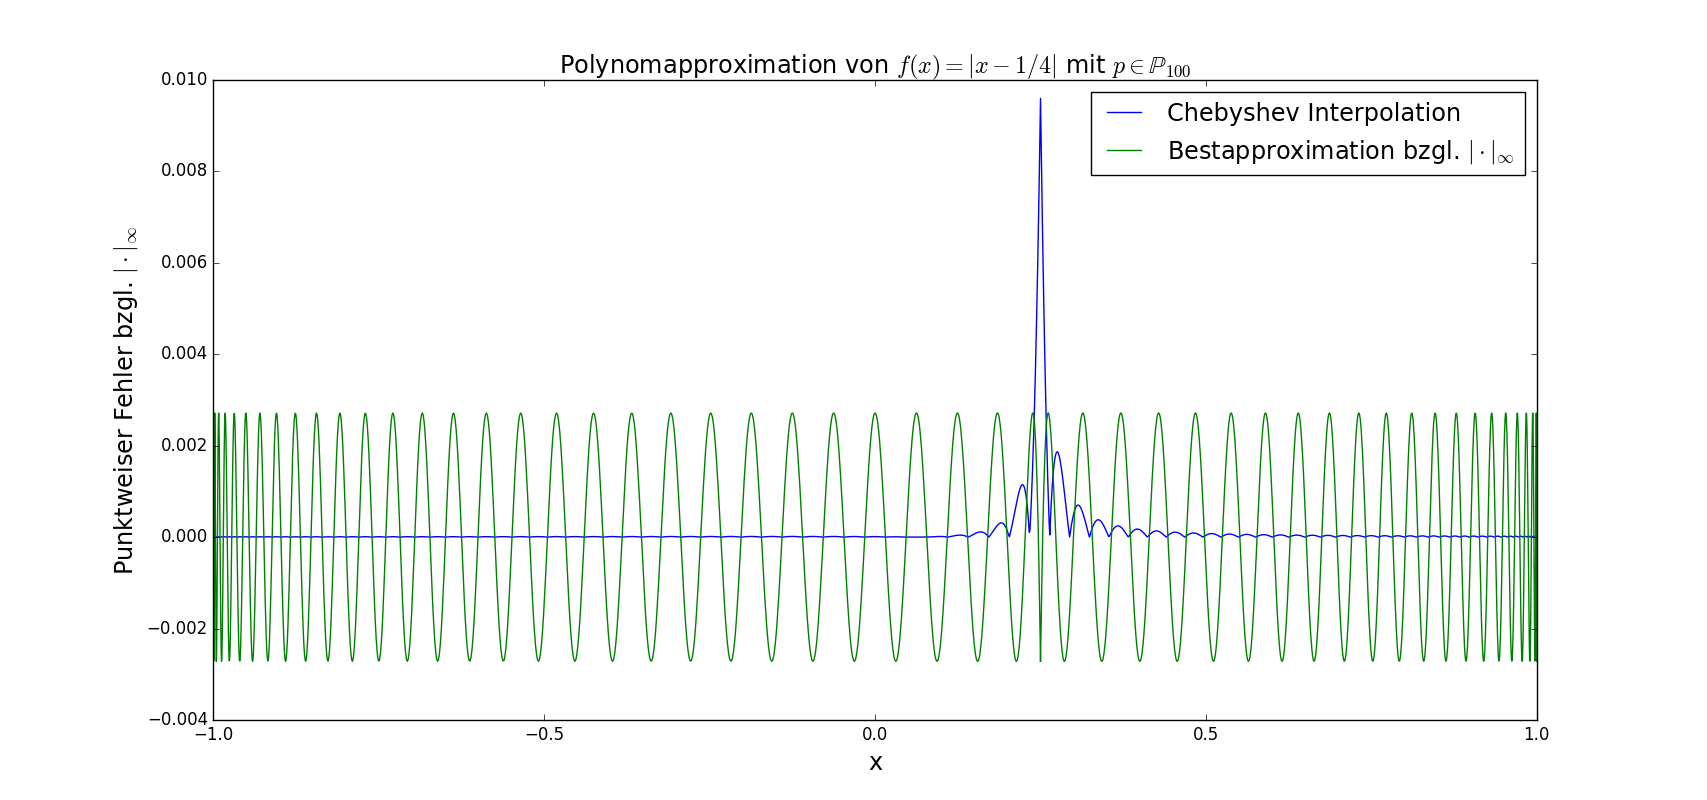
\includegraphics[width=\linewidth]{Figures/polynomial_approx_comparison.png}
 \caption{Visualisierung der Fehler verschiedener Approximationen, angelehnt an \autocite{Trefethen}. Hierbei wurde die Bestapproximation mithilfe des \emph{Remez} Algorithmus aus dem Chebfun Projekt (http://www.chebfun.org/) berechnet. Der Fehler der Chebyshev Approximation nimmt zu den Rändern hin stark ab.}
 \label{polyapproxcomp}
\end{figure}
\end{mathbsp}
Wie schon bei der Bestapproximation bzgl. der Maximumsnorm erhält man auch für die verallgemeinerte Bestapproximation eine Konvergenzaussage. Für unbeschränktes $I$ sind die Beweise sehr aufwändig und beispielsweise in \autocite{CouHil53} zu finden. 
\begin{maththeorem}
Für jedes $f\in L_w^2(I)$ gilt
\[\lim\limits_{N\to\infty}\norm{f-P_Nf}_{L_w^2(I)}=0\]
\end{maththeorem}
Die Konvergenzordnung ist hierbei abhängig von der Regularität von $f$ und der Art der für die Projektion verwendeten Orthogonalpolynome. Man nennt diese Art der Konvergenz in der Literatur auch \emph{spektrale Konvergenz}, da die Konvergenzrate abhängig von der Glattheit der Funktion ist. Man muss also aufpassen eine hohe Approximationsordnung nicht mit einer hohen Approximationsgenauigkeit zu verwechseln.\\
Für das Beispiel der Legendre Polynome, also mit konstanter Gewichtsfunktion $w$, zeigt Xiu in \autocite[Theorem 3.6]{dongbinxiu2010} folgendes Ergebnis
\begin{maththeorem}
\label{spectralconvth}
Für jedes $f\in H_w^p[-1,1]\coloneqq \left\lbrace v\colon I\to\R | \frac{d^mv}{dx^m}\in L_w^2(I),0\le m\le p\right\rbrace$ mit $p\ge 0, w\equiv 1$ gibt es eine Konstante $C$ unabhängig von $N$, so dass
\[\norm{f-P_Nf}_{L_w^2[-1,1]}\le CN^{-p}\norm{f}_{H_w^p[-1,1]}\]
\end{maththeorem}
\begin{mathbsp}
Als Veranschaulichung von Satz \ref{spectralconvth} approximieren wir verschiedene Funktionen $f\colon [-1,1]\to\R$ durch die orthogonale Projektion $P_Nf$ für steigendes $N\in\N$. In Abbildung \ref{figurespectralconverg} sind dafür die Fehler der Approximationen dargestellt. Dabei sind die $f$ unterschiedlich glatt und man erkennt unterschiedliche Konvergenzordnungen. Insbesondere erahnt man für die analytische Funktion $f(x)=\sin(\pi x)$ exponentielle Konvergenz in $N$. Da der General-Purpose Integrator, der für die Berechnung der Fourierkoeffizienten verwendet wurde für zu hohe Polynomgrade versagt, bricht die Darstellung an der entsprechenden Stelle ab.
\begin{figure}[h]
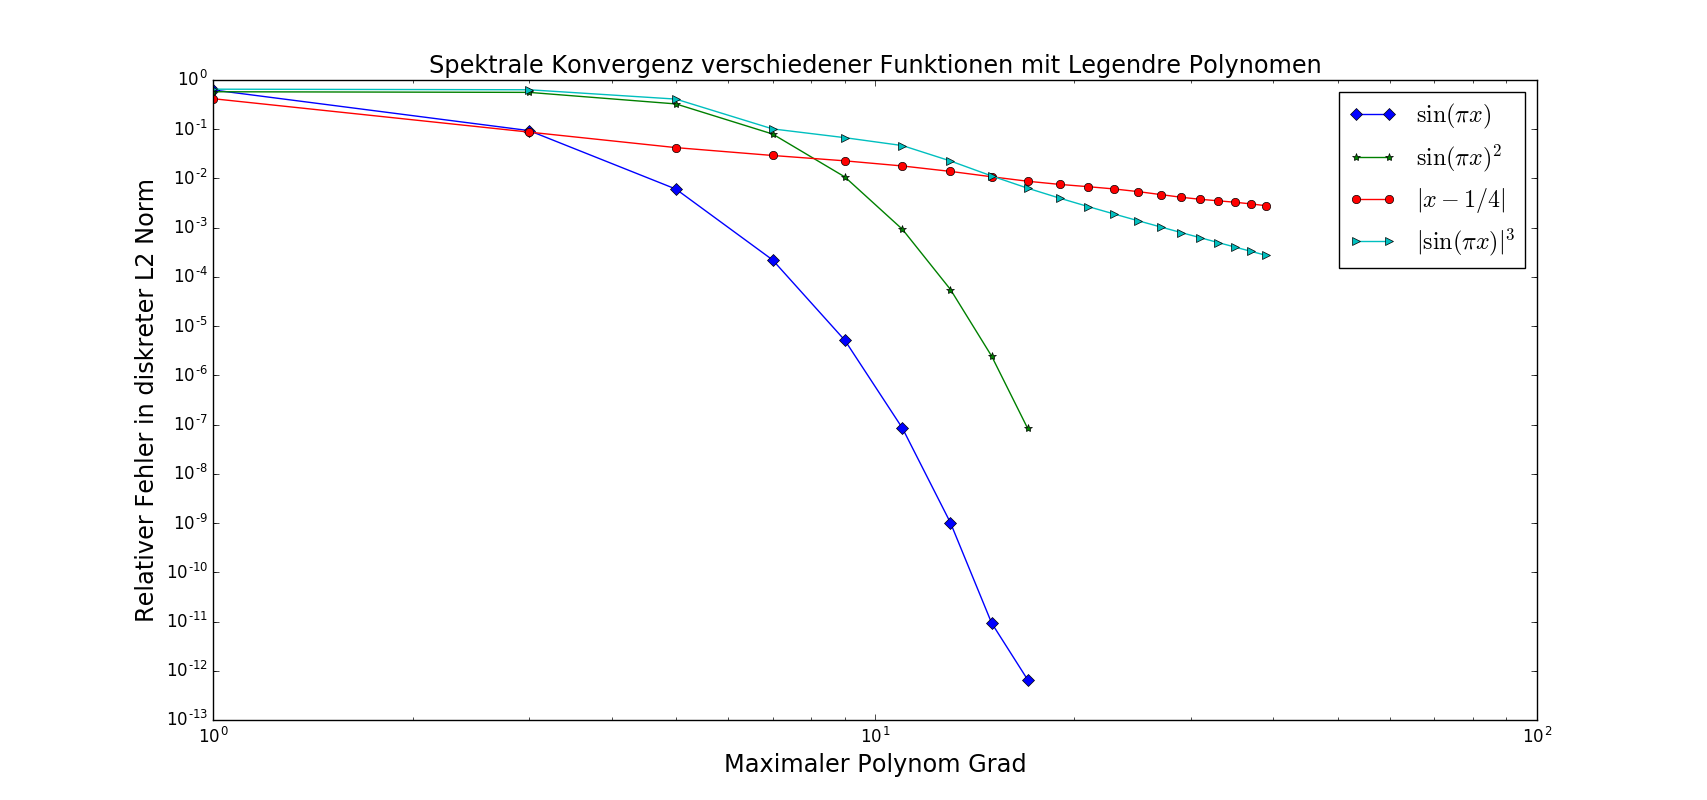
\includegraphics[width=\textwidth]{Figures/spectral_convergence_legendre.png}
\caption{Spektrale Konvergenz von Funktionen verschiedener Glattheit mithilfe von Legendre Polynomen und Gewichtsfunktion $w\equiv \onehalf$ auf $[-1,1]$.}
\label{figurespectralconverg}
\end{figure}
\end{mathbsp}